%!TEX program = xelatex
%!TEX options=--shell-escape
\documentclass[12pt]{article}

%
\usepackage[scheme=plain]{ctex}
%

\usepackage{fontspec}
%
\usepackage[margin = 1in]{geometry}

%
\usepackage[dvipsnames]{xcolor}

%
\usepackage{amsmath}
\usepackage{amssymb}
\usepackage{amsthm}
%
\usepackage{tensor}
%
\usepackage{slashed}
\usepackage{physics}

%
\usepackage{mathtools}

%
\usepackage{bm}
\newcommand{\dbar}{\dif\hspace*{-0.18em}\bar{}\hspace*{0.2em}}
\DeclareMathAlphabet\mathbfcal{OMS}{cmsy}{b}{n}
%\usepackage{bbold}
\newcommand*{\dif}{\mathop{}\!\mathrm{d}}
\newcommand*{\euler}{\mathrm{e}}
\newcommand*{\imagi}{\mathrm{i}}

\renewcommand{\vec}[1]{\boldsymbol{\mathbf{#1}}}

\usepackage{caption}
\usepackage{multirow}
\usepackage{enumitem}

%
\usepackage{mathrsfs}
\usepackage{dsfont}

%
\usepackage{hyperref}
\hypersetup{
    colorlinks=true,
    linkcolor=violet,
    filecolor=blue,      
    urlcolor=blue,
    citecolor=cyan,
}

%
\usepackage{graphicx}
\usepackage{subfig}
%
\graphicspath{{figures/}{../figures/}}

%
\usepackage{indentfirst}
%
\setlength{\parindent}{2em}
\linespread{1.25}

% 
% \setmainfont{Times New Roman}
\usepackage[T1]{fontenc}
\title{Note}
\author{Feng-Yang Hsieh}
\date{}

\begin{document}
\maketitle


\section{Signal}% (fold)
\label{sec:signal}
	We consider a simple extension of the standard model (SM)~\cite{Chen:2022vac}, which includes a vector-like dark fermion $(\overline{\chi}, \chi)$ and a complex singlet scalar $S$. A signature of CP violation could come from the Higgs-to-Higgs decays, $h_3 \to h_2h_1$, where $h_3 / h_2 / h_1$ are the heaviest scalar, second heaviest scalar, and the SM-like 125 GeV Higgs, respectively.

	The signal process is the triple production of 125 GeV Higgs bosons via the gluon fusion: 
	\[
		g g \to h_3 \to h_2 h_1 \to h_1h_1h_1
	\] 
	The Higgs boson $h_1$ would further decay to the $b \overline{b}$ pair. We consider the banchmark point 1 (BP1), where $m_{h_3} = \text{450 GeV}, m_{h_2} = \text{280 GeV}, m_{h_1} = \text{125 GeV}$. This process is generated at $\sqrt{s} = \text{13 TeV}$. Following are the MadGraph scripts for generating signal samples:
	\begin{verbatim}
		import model cxSM_VLF_EFT
		generate g g > h h h
		output MG5/gghhh_bsm
		launch MG5/gghhh_bsm

		shower=Pythia8
		detector=Delphes
		analysis=OFF
		madspin=ON
		done

		set param_card mh1 125
		set param_card mh2 280
		set param_card mh3 420
		set param_card theta12 0.73
		set param_card theta13 1.67079632679
		set param_card theta23 -0.73
		set param_card vs 200
		set param_card delta2 0
		set param_card Rdelta3 0
		set param_card Idelta3 -3.5
		set param_card b2 0
		set param_card Rc1 0
		set param_card Ic1 0
		set param_card Rc2 0
		set param_card Ic2 0
		set param_card Rd3 0
		set param_card Id3 0
		set param_card msq -5033.406281907266
		set param_card lam 0.13850082540690806
		set param_card Rdelta1 -47.561525227572744
		set param_card Idelta1 853.05384671134
		set param_card Rb1 -70476.6380004269
		set param_card Ib1 -30486.140015405872
		set param_card Rd1 -2.562109886826132
		set param_card Id1 2.257859679994403
		set param_card d2 6.340799300844676
		set param_card gh1ggr -0.00005478952893059635
		set param_card gh1gagar -0.00003270447254456052
		set param_card gh1Zgar -0.00005871986046374793
		set param_card gh2ggr -1.4279972541632635e-7
		set param_card gh2gagar -8.237715486808595e-8
		set param_card gh2Zgar -1.3984990232267825e-7
		set param_card gh3ggr -6.031835872118092e-6
		set param_card gh3gagar -1.1377279177203616e-6
		set param_card gh3Zgar -2.2999597941282603e-6

		set param_card decay 102 auto
		set param_card decay 103 auto

		set run_card nevents 100000
		set run_card ebeam1 6500.0
		set run_card ebeam2 6500.0

		set run_card ptb 24
		set run_card etab 2.6

		set spinmode none
		decay h > b b~

		done
	\end{verbatim}
% section signal (end)
\section{SPANet pairing}% (fold)
\label{sec:spanet_pairing}
	We employ the novel neural network structure \textsc{Spa-Net}~\cite{PhysRevD.105.112008, Fenton:2023ikr, 10.21468/SciPostPhys.12.5.178} to identify the correct pairings among the jets in the final states.
	\subsection{Training dataset preparation}% (fold)
	\label{sub:training_dataset_preparation}
		Preselection: $\ge 6$ jets with transverse momentum $p_{\text{T}} \ge \text{25 GeV}$ in range $\abs{\eta} < 2.5$.

		The input features for the \textsc{Spa-Net} are a list of jets, each represented by its 4-component vector $(p_\text{T}, \eta, \phi, m)$ as well as a boolean $b$-tag. We only keep each event's 15 highest $p_\text{T}$ jets. We define the correct jet assignments for each event by matching the jets to the simulated truth quarks within an angular distance of $\Delta R < 0.4$. Such an event will be dropped if a simulated truth quark is matched to more than one jet. Furthermore, some simulated truth quarks may not be matched to any jet, so the event will not be used in training either. 

		After the selection and matching, we could obtain the following results from 1M events:
		\begin{itemize}
			\item Total sample size: 522,899
			\item 1h sample size: 184,769
			\item 2h sample size: 161,476
			\item 3h sample size: 94,464
		\end{itemize}
		Here, the 1h sample is where we could define the correct jet assignments for 1 Higgs boson. 
	% subsection training_dataset_preparation (end)
	\subsection{Training results}% (fold)
	\label{sub:training_results}
		\begin{itemize}
			\item Training sample:
			\begin{itemize}
				\item Total sample size: 470,609
				\item 1h sample size: 166,490
				\item 2h sample size: 145,309
				\item 3h sample size: 84,913
				\item 5\% used on validation
			\end{itemize}
			\item Testing sample: 
			\begin{itemize}
				\item Total sample size: 52,290
				\item 1h sample size: 18,279
				\item 2h sample size: 16,167
				\item 3h sample size: 9,551
			\end{itemize}
		\end{itemize}

		Some useful definitions for evaluating jet assignment performance:
		\begin{itemize}		
		\item Event Efficiency
		\begin{equation}
			\epsilon^{\text{event}} \equiv \frac{\text{number of events with and all Higgs are correctly identified}}{\text{number of events}} 
		\end{equation}

		\item Higgs Efficiency
		\begin{equation}
			\epsilon^{\text{h}} \equiv \frac{\text{number of correctly identified Higgs}}{\text{number of identifiable Higgs}} 
		\end{equation}
	\end{itemize}
		The training results are shown in Table~\ref{tab:SPANet_triHiggs_0b}.
		\begin{table}[htpb]
			\centering
			\caption{\textsc{Spa-Net} pairing efficiencies on 3h events.}
			\label{tab:SPANet_triHiggs_0b}
			\begin{tabular}{c|c|cc}
				$N_\text{Jet}$ & Event Fraction & Event Efficiency & Higgs Efficiency \\
				\hline
				$=6$	  &   0.077             &    0.532              &    0.650             \\
				$=7$	  &   0.057             &    0.345              &    0.536             \\
				$\ge 8$	  &   0.052             &    0.237              &    0.452             \\
				Total	  &   0.186             &    0.375              &    0.548   
			\end{tabular}
		\end{table}
	% subsection training_results (end)
% section spanet_pairing (end)
\section{\texorpdfstring{$\chi^2$}{chi2} pairing}% (fold)
\label{sec:chi2_pairing}
	$\chi^2$ method considers all possible combinations of final jets and selects the configuration that minimizes the mass difference between Higgs candidates and SM Higgs, i.e., minimizes this:
	\begin{equation}\label{eq:triHiggs_chisq}
		\chi^2 = [m(j_1j_2) - m_h]^2 + [m(j_3j_4) - m_h]^2 + [m(j_5j_6) - m_h]^2
	\end{equation}
	where $m(j_ij_j)$ is the invariant mass of jet $i, j$ and $m_h = \text{125 GeV}$.

	Table~\ref{tab:chi2_pairing_triHiggs_0b} is the performance of the $\chi^2$ method.
	\begin{table}[htpb]
		\centering
		\caption{$\chi^2$ pairing efficiencies on 3h events.}
		\label{tab:chi2_pairing_triHiggs_0b}
		\begin{tabular}{c|c|cc}
			$N_\text{Jet}$ & Event Fraction & Event Efficiency & Higgs Efficiency \\
			\hline
			$=6$	  &   0.077             &    0.403              &    0.450             \\
			$=7$	  &   0.057             &    0.158              &    0.281             \\
			$\ge 8$	  &   0.052             &    0.000              &    0.077             \\
			Total	  &   0.186             &    0.215              &    0.294
		\end{tabular}
	\end{table}
% section chi2_pairing (end)
\section{Estimate cross-section of background process}% (fold)
\label{sec:estimate_cross_section_of_background_process}
	Besides the 6 $b$ background, we need to consider the backgrounds that come from the mis-tagging of light jets or charm-jets to $b$-jets. We assume that the probability of a charm-jet being misidentified as $b$-jet is $\mathcal{P}_{c\to b} = 0.1$ and that of light jets is $\mathcal{P}_{j\to b} = 0.01$. The $b$-tagging efficiency is assumed to be $\mathcal{P}_{b\to b} = 0.7$.

	Table~\ref{tab:cross_section_of_mis_tagging_background} shows the cross-section computed from \verb|MadGraph| and the cross-section times the mis-tagging probabilities $\mathcal{P}_{c\to b}$ and $\mathcal{P}_{j\to b}$. Table~\ref{tab:cross_section_of_mis_tagging_background_w_cuts} shows the same results with kinetic cuts. We require the transverse momentum $p_{\text{T}}$ of each jet greater than $\text{24 GeV}$ and in the range $\abs{\eta} < 2.6$ at the \verb|MadGraph| level. The $6b$ process contributes much more than the processes containing charm jets and light jets.
	\begin{table}[htpb]
		\centering
		\caption{The cross-sections of $6b$ and mis-tagging background processes. The cross-sections are computed from the MadGraph at $\sqrt{s} = 13 \text{ TeV}$.}
		\label{tab:cross_section_of_mis_tagging_background}
		\begin{tabular}{c|cc}
		process                                         & $\sigma\text{ (pb)}$ & $\sigma\times\mathcal{P}(\text{tagging efficiency})\text{ (pb)}$ \\ \hline
		$(b\overline{b})(b\overline{b})(b\overline{b})$ & $2.53 \times 10^{3}$ & $2.97 \times 10^{2}$                                             \\
		$(b\overline{b})(b\overline{b})(c\overline{c})$ & $2.72 \times 10^{2}$ & $6.54 \times 10^{-1}$                                            \\
		$(b\overline{b})(c\overline{c})(c\overline{c})$ & $3.73 \times 10^{1}$ & $1.83 \times 10^{-3}$                                            \\
		$(b\overline{b})(b\overline{b})(jj)$            & $7.44 \times 10^{4}$ & 1.79
		\end{tabular}
	\end{table}

	\begin{table}[htpb]
		\centering
		\caption{The cross-sections of $6b$ and mis-tagging background processes. The cross-sections are computed from the MadGraph at $\sqrt{s} = 13 \text{ TeV}$. We require the transverse momentum $p_{\text{T}}$ of each jets greater than $\text{24 GeV}$ in range $\abs{\eta} < 2.6$.}
		\label{tab:cross_section_of_mis_tagging_background_w_cuts}
		\begin{tabular}{c|cc}
		process                                         & $\sigma\text{ (fb)}$ & $\sigma\times\mathcal{P}(\text{tagging efficiency})\text{ (fb)}$ \\ \hline
		$(b\overline{b})(b\overline{b})(b\overline{b})$ & $9.63 \times 10^{2}$ & $113.35$                                                         \\
		$(b\overline{b})(b\overline{b})(c\overline{c})$ & $1.67 \times 10^{3}$ & $4.02$                                                           \\
		$(b\overline{b})(c\overline{c})(c\overline{c})$ & $1.06 \times 10^{3}$ & $5.19 \times 10^{-2}$                                            \\
		$(b\overline{b})(b\overline{b})(jj)$            & $4.16 \times 10^{5}$ & $9.98$                                                           \\
		$(b\overline{b})(jj)(jj)$                       & $1.50 \times 10^{7}$ & $7.73 \times 10^{-2}$                                           
		\end{tabular}
	\end{table}
% section estimate_cross_section_of_background_process (end)
\section{Compute pairing efficiency}% (fold)
\label{sec:compute_pairing_efficiency}
	To understand the pairing performance with different pairing methods, we compute how many events where 1h/2h/3h bosons are reconstructed correctly.

	The pairing performance of \textsc{Spa-Net} are shown in Table~\ref{tab:SPANet_triHiggs_0b_1h2h3h}. Table~\ref{tab:chi2_pairing_triHiggs_0b_1h2h3h} is the performance of the $\chi^2$ method. For both cases, we found the number of events where only two Higgs are paired correctly is tiny, which means if we can pair two Higgs bosons correctly, then we have a high chance to pair the final Higgs correctly.

	Note that Higgs Efficiencies of \textsc{Spa-Net} are inconsistent with Table~\ref{tab:SPANet_triHiggs_0b}. This issue needs more checking.
	\begin{table}[htpb]
		\centering
		\caption{\textsc{Spa-Net} pairing efficiencies on different categories.}
		\label{tab:SPANet_triHiggs_0b_1h2h3h}
		\begin{tabular}{c|cccc|c}
			\multicolumn{1}{l|}{} & \multicolumn{4}{c|}{Correctly reconstructed Higgs} & \multicolumn{1}{l}{} \\ \hline
			$N_\text{Jet}$        & 3h          & 2h         & 1h         & 0h         & Higgs Efficiency     \\ \hline
			$=6$                  & 0.532       & 0.000      & 0.119      & 0.348      & 0.572                \\
			$=7$                  & 0.345       & 0.021      & 0.166      & 0.469      & 0.414                \\
			$\ge 8$               & 0.237       & 0.022      & 0.186      & 0.554      & 0.314                \\ \hline
			Total                 & 0.375       & 0.014      & 0.156      & 0.455      & 0.436               
		\end{tabular}
	\end{table}
	\begin{table}[htpb]
		\centering
		\caption{$\chi^2$ pairing efficiencies on different categories.}
		\label{tab:chi2_pairing_triHiggs_0b_1h2h3h}
		\begin{tabular}{c|cccc|c}
			\multicolumn{1}{l|}{} & \multicolumn{4}{c|}{Correctly reconstructed Higgs} & \multicolumn{1}{l}{} \\ \hline
			$N_\text{Jet}$        & 3h          & 2h         & 1h         & 0h         & Higgs Efficiency     \\ \hline
			$=6$                  & 0.403       & 0.000      & 0.143      & 0.455      & 0.450                \\
			$=7$                  & 0.158       & 0.070      & 0.228      & 0.544      & 0.281                \\
			$\ge 8$               & 0.000       & 0.000      & 0.231      & 0.769      & 0.077                \\ \hline
			Total                 & 0.215       & 0.022      & 0.194      & 0.570      & 0.294               
		\end{tabular}
	\end{table}
% section compute_pairing_efficiency (end)
\section{SPANet pairing and classification}% (fold)
\label{sec:spanet_pairing_and_classification}
	
	We train a \textsc{Spa-Net} to identify the correct pairings and perform the signal/background classification at the same time.

	\subsection{Training dataset}% (fold)
	\label{sub:training_dataset_classification}
		The selection and matching process for the jet pairing is the same as Section~\ref{sub:training_dataset_preparation}. We prepare the signal and background samples of the same size for classification.

		For the jet assignment part,
		\begin{itemize}
			\item Training sample:
			\begin{itemize}
				\item Total sample size: 1,800,000
				\item 1h sample size: 318,053
				\item 2h sample size: 277,876
				\item 3h sample size: 162,444
				\item 5\% used on validation
			\end{itemize}
			\item Testing sample:
			\begin{itemize}
				\item Total sample size: 200,000
				\item 1h sample size: 35,372
				\item 2h sample size: 30,853
				\item 3h sample size: 18,004
			\end{itemize}
		\end{itemize}

		For event classification,
		\begin{itemize}
			\item Training sample:
			\begin{itemize}
				\item Total sample size: 1,800,000
				\item Signal sample size: 900,000
				\item Background sample size: 900,000
				\item 5\% used on validation
			\end{itemize}
			\item Testing sample:
			\begin{itemize}
				\item Total sample size: 200,000
				\item Signal sample size: 100,000
				\item Background sample size: 100,000
			\end{itemize}
		\end{itemize}

		This training takes around 10 hours on our server.
	% subsection training_dataset_classification (end)
	\subsection{Training results}% (fold)
	\label{sub:training_results}
		The training results are presented in Table \ref{tab:SPANet_triHiggs_0b_cls_pairing_results}. This result is better than Table~\ref{tab:SPANet_triHiggs_0b_1h2h3h} since we use larger training datasets.

		\begin{table}[htpb]
			\centering
			\caption{\textsc{Spa-Net} training results on the tri-Higgs samples. \textsc{Spa-Net} is trained on jet pairing and event classification tasks at the same time.}
			\label{tab:SPANet_triHiggs_0b_cls_pairing_results}
			\begin{tabular}{c|cccc|c}
			\multicolumn{1}{l|}{} & \multicolumn{4}{c|}{Correctly reconstructed Higgs} & \multicolumn{1}{l}{} \\ \hline
			$N_\text{Jet}$        & 3h          & 2h         & 1h         & 0h         & Higgs Efficiency     \\ \hline
			$=6$                  & 0.656       & 0.000      & 0.082      & 0.262      & 0.684                \\
			$=7$                  & 0.436       & 0.017      & 0.168      & 0.379      & 0.504                \\
			$\ge 8$               & 0.341       & 0.018      & 0.173      & 0.468      & 0.411                \\ \hline
			Total                 & 0.478       & 0.012      & 0.142      & 0.368      & 0.533               
			\end{tabular}
			
		\end{table}

		Table \ref{tab:SPANet_triHiggs_0b_cls_classification_results} presents the classification training results. We use the accuracy (ACC) and the area under the Receiver Operating Characteristic (ROC) curve (AUC) as two metrics.
		\begin{table}[htpb]
			\centering
			\caption{The \textsc{Spa-Net} classification training results with tri-Higgs sample.}
			\label{tab:SPANet_triHiggs_0b_cls_classification_results}
			\begin{tabular}{c|cc}
				             & ACC     & AUC      \\ \hline
			\textsc{Spa-Net} & $0.822$ & $0.900 $
			\end{tabular}
		\end{table}
	% subsection training_results (end)
	\subsection{3h training dataset}% (fold)
	\label{sub:3h_training_dataset}
		We only consider 3h events in pairing tasks in this subsection. We prepare the signal and background samples of the same size for classification.

		For the jet assignment part,
		\begin{itemize}
			\item Training sample:
			\begin{itemize}
				\item Total sample size: 1,800,000
				\item 1h sample size: 0
				\item 2h sample size: 0
				\item 3h sample size: 900,000
				\item 5\% used on validation
			\end{itemize}
			\item Testing sample:
			\begin{itemize}
				\item Total sample size: 200,000
				\item 1h sample size: 0
				\item 2h sample size: 0
				\item 3h sample size: 100,000
			\end{itemize}
		\end{itemize}

		For event classification,
		\begin{itemize}
			\item Training sample:
			\begin{itemize}
				\item Total sample size: 1,800,000
				\item Signal sample size: 900,000
				\item Background sample size: 900,000
				\item 5\% used on validation
			\end{itemize}
			\item Testing sample:
			\begin{itemize}
				\item Total sample size: 200,000
				\item Signal sample size: 100,000
				\item Background sample size: 100,000
			\end{itemize}
		\end{itemize}

		The training results are presented in Table \ref{tab:SPANet_triHiggs_0b_3h_cls_pairing_results}. This result is similar to Table~\ref{tab:SPANet_triHiggs_0b_cls_pairing_results}.

		\begin{table}[htpb]
			\centering
			\caption{\textsc{Spa-Net} training results on the tri-Higgs samples, where we only consider 3h events. \textsc{Spa-Net} is trained on jet pairing and event classification tasks at the same time.}
			\label{tab:SPANet_triHiggs_0b_3h_cls_pairing_results}
			\begin{tabular}{c|cccc|c}
			\multicolumn{1}{l|}{} & \multicolumn{4}{c|}{Correctly reconstructed Higgs} & \multicolumn{1}{l}{} \\ \hline
			$N_\text{Jet}$        & 3h          & 2h         & 1h         & 0h         & Higgs Efficiency     \\ \hline
			$=6$                  & 0.680       & 0.000      & 0.084      & 0.236      & 0.708                \\
			$=7$                  & 0.477       & 0.014      & 0.150      & 0.359      & 0.536                \\
			$\ge 8$               & 0.311       & 0.027      & 0.184      & 0.477      & 0.391                \\ \hline
			Total                 & 0.491       & 0.014      & 0.139      & 0.356      & 0.547               
			\end{tabular}
			
		\end{table}

        However, some issues should be resolved when we try to use all 3h events for combining training. The loss values are not reasonable.
	% subsection 3h_training_dataset (end)
% section spanet_pairing_and_classification (end)
\section{Review the pairing methods}% (fold)
\label{sec:review_the_pairing_methods}
	In Refs.~\cite{Papaefstathiou:2019ofh, Papaefstathiou:2023uum}: We select the 6 $b$-tagged jets with the highest transverse momentum. The requirements for the transverse momentum and pseudo-rapidity are applied. We subsequently make use of the observable:
	\begin{equation}
		\chi^{2,(6)} = \sum_{qr\in J} (m_{qr} - m_h)^2
	\end{equation}
	where $J = \{j_1j_2,j_3j_4,j_5j_6\} $ is the set of all possible 15 pairings of 6 $b$-tagged jets. Out of all the possible combinations we pick the one with the smallest value $\chi_{\text{min}}^{2,(6)}$. The pairing of $b$-jets defining $\chi_{\text{min}}^{2,(6)}$ is our best candidate for the reconstruction of the three Higgs bosons, $h$. No pairing efficiency is provided.

	In Ref.~\cite{Papaefstathiou:2020lyp}: We select the 6 $b$-tagged jets with the highest transverse momentum and form pairs in different combinations, with the aim of first reconstructing individual SM-like Higgs bosons, $h_1$, and subsequently the two scalars $h_2$ and $h_3$. To this end, we introduce two observables:
	\begin{equation}
		\chi^{2,(4)} = \sum_{qr\in I} (m_{qr} - m_h)^2
	\end{equation}
	\begin{equation}
		\chi^{2,(6)} = \sum_{qr\in J} (m_{qr} - m_h)^2
	\end{equation}
	where we have defined the sets $I = \{i_1i_2,i_3i_4\}$ and $J = \{j_1j_2,j_3j_4,j_5j_6\}$, constructed from different pairings of 4 and 6 $b$-tagged jets, respectively, and where $m_{qr}$ denotes the invariant mass of the respective pairing, $qr$. Note that the set $I$ that defines $\chi_{\text{min}}^{2,(4)}$ should be a subset of the arrangement $J$.

	We select the combinations of $b$-tagged jets entering in $I$ and $J$ based on the minimization of the sum
	\begin{equation}
		\chi^{2,(4)} + \chi^{2,(6)}
	\end{equation}
	We then ``identify'' candidates for the scalars $h_2$ and $h_3$ with the pairing configurations $I_{\text{min}}$ and $J_{\text{min}}$ which minimise $\chi^{2,(4)}$ and $\chi^{2,(6)}$ respectively. Note that this procedure does not guarantee that $I_{\text{min}}$ indeed reconstructs to $h_2$; in fact, we found this to be the case in about 40\% on average for all benchmark samples, being slightly higher than a ``blind guess'' that would lead to a probability of 1/3.

% section review_the_pairing_methods (end)
\section{6b requirement}% (fold)
\label{sec:6b_requirement}
	They could utilize stronger kinetic and $b$-tagging requirements in experiments. However, we do not use the $b$-tag information for the previous $\chi^2$ method. Thus, we change the preselection condition to make a fair comparison.

	For testing samples, we only consider the event that contains at least 6 $b$-tagged jets. The Higgs Bosons are reconstructed by pairing the 6 leading $b$-jets for the $\chi^2$ method. Thus, the best one is chosen from 15 possible pairing combinations.

	Table~\ref{tab:chi2_pairing_triHiggs_6b_3h} and Table~\ref{tab:SPANet_triHiggs_6b_3h} are the pairing performance on 6 $b$-tagged samples. The $\chi^2$ method performs better than the previous results (Table~\ref{tab:chi2_pairing_triHiggs_0b_1h2h3h}) but still performs worse than the \textsc{Spa-Net} pairing.
	\begin{table}[htpb]
		\centering
		\caption{$\chi^2$ pairing efficiencies on different categories. The $\chi^2$ method only considers the 6 leading $b$-jets.}
		\label{tab:chi2_pairing_triHiggs_6b_3h}
		\begin{tabular}{c|cccc|c}
			\multicolumn{1}{l|}{} & \multicolumn{4}{c|}{Correctly reconstructed Higgs} & \multicolumn{1}{l}{} \\ \hline
			$N_\text{Jet}$        & 3h          & 2h         & 1h         & 0h         & Higgs Efficiency     \\ \hline
			$=6$                  & 0.500       & 0.000      & 0.124      & 0.376      & 0.541                \\
			$=7$                  & 0.322       & 0.072      & 0.185      & 0.486      & 0.389                \\
			$\ge 8$               & 0.238       & 0.026      & 0.156      & 0.579      & 0.308                \\ \hline
			Total                 & 0.329       & 0.013      & 0.159      & 0.499      & 0.391               
		\end{tabular}
	\end{table}
	\begin{table}[htpb]
		\centering
		\caption{\textsc{Spa-Net} training results on the tri-Higgs samples, where we only consider 3h events. \textsc{Spa-Net} is trained on $\ge 0b$ datasets and tested on $\ge 6b$ datasets.}
		\label{tab:SPANet_triHiggs_6b_3h}
		\begin{tabular}{c|cccc|c}
			\multicolumn{1}{l|}{} & \multicolumn{4}{c|}{Correctly reconstructed Higgs} & \multicolumn{1}{l}{} \\ \hline
			$N_\text{Jet}$        & 3h          & 2h         & 1h         & 0h         & Higgs Efficiency     \\ \hline
			$=6$                  & 0.679       & 0.000      & 0.074      & 0.246      & 0.704                \\
			$=7$                  & 0.522       & 0.013      & 0.127      & 0.337      & 0.574                \\
			$\ge 8$               & 0.354       & 0.019      & 0.180      & 0.447      & 0.427                \\ \hline
			Total                 & 0.492       & 0.013      & 0.136      & 0.359      & 0.546               
		\end{tabular}
	\end{table}
% section 6b_requirement (end)
\section{Another pairing method}% (fold)
\label{sec:another_pairing_method}
	The pairing algorithm is defined to minimize
	\begin{equation}\label{eq:pairing_method_abs}
		\abs{m_{h_1} - 120} + \abs{m_{h_2} - 115} + \abs{m_{h_3} - 110}
	\end{equation}
	where $m_{h_i}$ is the mass of the $i$-th Higgs boson candidate (sorted by $p_{\text{T}}$) in units of GeV. The numbers in this definition are chosen based on the peaks of the $m_{h_i}$ distributions in simulated signal events.

	Figure~\ref{fig:mh_distribution_6b} is the Higgs boson invariant mass $m_h$ distributions. The peaks of the $m_{h}$ distributions in our simulation are $121, 119, 116 \text{ GeV}$. Based on these values we modify the numbers in Equation~\ref{eq:pairing_method_abs}.
	\begin{figure}[htpb] 
		\centering
        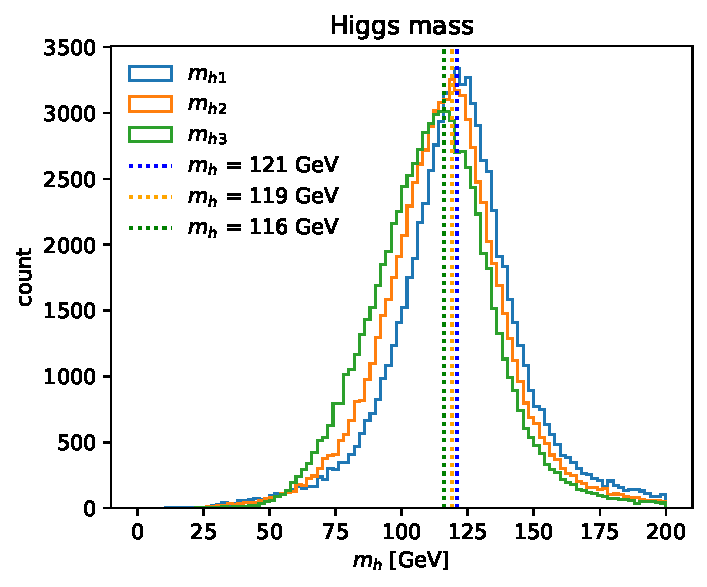
\includegraphics[width=0.65\textwidth]{mh_distribution_6b.pdf} 
		\caption{The Higgs boson mass distributions. Here, we only consider the event containing at least 6 $b$-tagged jets.}
		\label{fig:mh_distribution_6b}
	\end{figure}
	Table~\ref{tab:chi2_abs_pairing_triHiggs_6b_3h} is the pairing performance on 6 $b$-tagged samples. The absolute value method performs worse than the $\chi^2$ method (Table~\ref{tab:chi2_pairing_triHiggs_6b_3h}).
	\begin{table}[htpb]
		\centering
		\caption{$\chi^2$ pairing efficiencies on different categories. The $\chi^2$ method only considers the 6 leading $b$-jets.}
		\label{tab:chi2_abs_pairing_triHiggs_6b_3h}
		\begin{tabular}{c|cccc|c}
			\multicolumn{1}{l|}{} & \multicolumn{4}{c|}{Correctly reconstructed Higgs} & \multicolumn{1}{l}{} \\ \hline
			$N_\text{Jet}$        & 3h          & 2h         & 1h         & 0h         & Higgs Efficiency     \\ \hline
			$=6$                  & 0.476       & 0.000      & 0.135      & 0.388      & 0.522                \\
			$=7$                  & 0.293       & 0.011      & 0.185      & 0.511      & 0.362                \\
			$\ge 8$               & 0.215       & 0.026      & 0.168      & 0.589      & 0.289                \\ \hline
			Total                 & 0.303       & 0.015      & 0.167      & 0.515      & 0.367               
		\end{tabular}
	\end{table}
% section another_pairing_method (end)
\section{New simulation setting}% (fold)
\label{sec:new_simulation_setting}
    We apply the new setting to the event generation for a fair comparison. Following are the notes about the latest simulation setting.

    The $6b$ analysis uses $R = 0.4$ anti-$k_{\text{T}}$ jets. All jets are required to have $p_{\text{T}} > 20 \text{ GeV}$ and  $\abs{\eta} < 2.5$, to be within the tracker acceptance for $b$-tagging. 

    All events must pass the Preselection. They must have at least six jets, defined by the earlier selection criteria. Of these 6 jets, at least 4 jets must have $p_{\text{T}} > \text{40 GeV}$ and at least 4 jets must be $b$-tagged.

    Pairing is performed on all events passing the Preselection. In the case of $4b$ or $5b$ events, the 6 jets considered for pairing into Higgs candidates are the $b$-tagged jets and the extra jets are selected as the highest $p_{\text{T}}$ of the remaining light-flavour jets. In the case of $6b$ events, the 6 jets are the 6 leading $p_{\text{T}}$ $b$-tagged jets.
% section new_simulation_setting (end)
\section{Pairing for new simulated samples}% (fold)
\label{sec:pairing_for_new_simulated_samples}
    We modified the \verb|Delphes| card to apply the anti-$k_{\text{T}}$ clustering algorithm with $R = 0.4$ and change the $b$-tagging efficiency to the ATLAS DL1r 77\% working point. At this working point, the light-jet (charm-jet) rejection is about 130 (4.9).

    Figure~\ref{fig:mh_distribution_new} is the Higgs boson invariant mass $m_h$ distributions for new simulated samples. All events passing the Preselection and matching are used to generate this plot. The peaks of the $m_{h}$ distributions in our simulation are $119, 115, 111 \text{ GeV}$. Based on these values we modify the numbers in Equation~\ref{eq:pairing_method_abs}.
	\begin{figure}[htpb] 
		\centering
        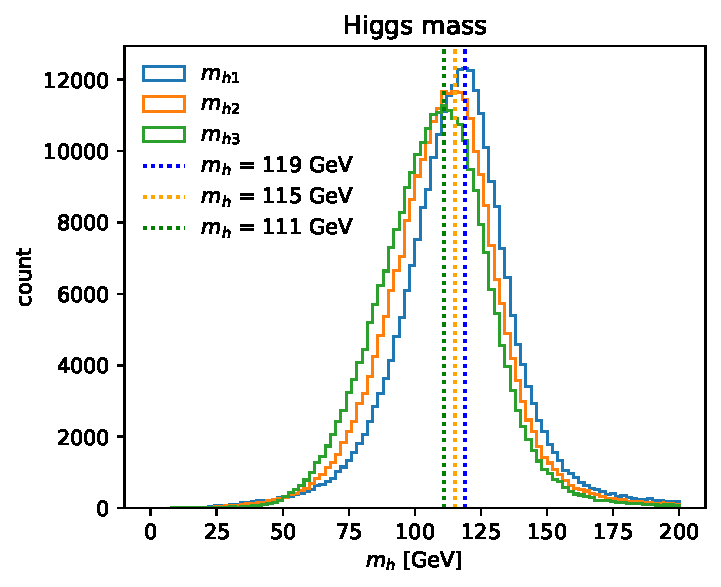
\includegraphics[width=0.65\textwidth]{mh_distribution_new.pdf}
		\caption{The Higgs boson mass distributions. Here, we consider all events passing the Preselection and the correct pairing can be obtained.}
		\label{fig:mh_distribution_new}
	\end{figure}

    Table~\ref{tab:chi2_pairing_triHiggs_3h_new}, \ref{tab:chi2_abs_pairing_triHiggs_3h_new} and \ref{tab:SPANet_triHiggs_3h_new} are the pairing performance on new simulated samples. The \textsc{Spa-Net} performs the best.
    \begin{table}[htpb]
		\centering
        \caption{$\chi^2$ pairing efficiencies on different categories. We minimize the quantity defined in Equation~\ref{eq:triHiggs_chisq}. The $\chi^2$ method considers the possible combinations of 6 jets.}
		\label{tab:chi2_pairing_triHiggs_3h_new}
		\begin{tabular}{c|c|cccc|c}
        \multicolumn{1}{l|}{} &          & \multicolumn{4}{c|}{Correctly reconstructed Higgs} & \multicolumn{1}{l}{} \\ \hline
        $N_\text{Jet}$        & Fraction & 3h          & 2h         & 1h         & 0h         & Higgs Efficiency     \\ \hline
        $=6$                  & 0.241    & 0.519       & 0.000      & 0.112      & 0.368      & 0.557                \\
        $=7$                  & 0.335    & 0.272       & 0.010      & 0.186      & 0.532      & 0.341                \\
        $\ge 8$               & 0.424    & 0.147       & 0.008      & 0.196      & 0.649      & 0.218                \\ \hline
        Total                 & 1.000    & 0.279       & 0.007      & 0.172      & 0.542      & 0.341               
		\end{tabular}
	\end{table}
    \begin{table}[htpb]
		\centering
		\caption{Absolute value pairing efficiencies on different categories. We minimize the quantity defined in Equation~\ref{eq:pairing_method_abs}. The absolute value method considers the possible combination of 6 jets.}
		\label{tab:chi2_abs_pairing_triHiggs_3h_new}
		\begin{tabular}{c|c|cccc|c}
			\multicolumn{1}{l|}{} &          & \multicolumn{4}{c|}{Correctly reconstructed Higgs} & \multicolumn{1}{l}{} \\ \hline
			$N_\text{Jet}$        & Fraction & 3h          & 2h         & 1h         & 0h         & Higgs Efficiency     \\ \hline
			$=6$                  & 0.241    & 0.457 & 0.000 & 0.131 & 0.412 &  0.500                \\
			$=7$                  & 0.335    & 0.239 & 0.009 & 0.184 & 0.568 &  0.306                \\
			$\ge 8$               & 0.424    & 0.136 & 0.007 & 0.197 & 0.661 &  0.206                \\ \hline
			Total                 & 1.000    & 0.248 & 0.006 & 0.176 & 0.570 &  0.311               
		\end{tabular}
	\end{table}
    \begin{table}[htpb]
		\centering
        \caption{\textsc{Spa-Net} training results on the tri-Higgs samples, where we only consider 3h events. The \textsc{Spa-Net} method considers all jets in the final state.}
		\label{tab:SPANet_triHiggs_3h_new}
		\begin{tabular}{c|c|cccc|c}
			\multicolumn{1}{l|}{} &          & \multicolumn{4}{c|}{Correctly reconstructed Higgs} & \multicolumn{1}{l}{} \\ \hline
			$N_\text{Jet}$        & Fraction & 3h          & 2h         & 1h         & 0h         & Higgs Efficiency     \\ \hline
			$=6$                  & 0.241    & 0.619 & 0.000 & 0.097 & 0.283 &  0.652                \\
			$=7$                  & 0.335    & 0.481 & 0.008 & 0.150 & 0.361 &  0.536                \\
			$\ge 8$               & 0.424    & 0.350 & 0.011 & 0.171 & 0.469 &  0.414                \\ \hline
			Total                 & 1.000    & 0.459 & 0.007 & 0.146 & 0.388 &  0.512               
		\end{tabular}
	\end{table}
% section pairing_for_new_simulated_samples (end)
\section{Modify the matching strategy}% (fold)
\label{sec:modify_the_matching_strategy}
    For the previous exercise, we define the correct jet assignments for each event by matching the jets to the simulated truth quarks within an angular distance of $\Delta R < 0.4$. Such an event will be dropped if a simulated truth quark is matched to more than one jet. Furthermore, some simulated truth quarks may not be matched to any jet, so the event will not be used in training either.

    We modify our strategy for more than one jet case. If more than one jet can be matched to a simulated truth quark in the $\Delta R=0.4$ cone, we choose the nearest one by the $\Delta R$ distance. This method is the same as the di-Higgs analysis~\cite{Stanislaus:2020vfx}.

    Table~\ref{tab:preselection_cutflow_number} is the cutflow number at different selection cuts.
    \begin{table}[htpb]
        \centering
        \caption{The number of passing events, efficiencies, and passing rates for signal processes at different selection cuts.}
        \label{tab:preselection_cutflow_number}
        \begin{tabular}{l|rrr}
                                                         & Count  & Efficiency & Pass rate \\ \hline
        Total                                            & 100000 & 1.00       & 1.00      \\
        $\ge 6$ jets                                     & 61454  & 0.61       & 0.61      \\
        $\ge 4$ jets with $p_{\text{T}} > \text{40 GeV}$ & 50341  & 0.82       & 0.50      \\
        $\ge 4$ $b$-jets                                 & 32337  & 0.64       & 0.32      \\ \hline
        Matching 3h                                      & 9944   & 0.31       & 0.10      \\
        Matching 2h                                      & 11341  & 0.35       & 0.11      \\
        Matching 1h                                      & 8941   & 0.28       & 0.09      \\
        \end{tabular}
    \end{table}

    Table~\ref{tab:chi2_pairing_triHiggs_3h_new_match} and \ref{tab:abs_pairing_triHiggs_3h_new_match} are the pairing performance with the new matching strategy. The results are similar to the previous one (Table~\ref{tab:chi2_pairing_triHiggs_3h_new} and \ref{tab:chi2_abs_pairing_triHiggs_3h_new}).
    \begin{table}[htpb]
		\centering
        \caption{$\chi^2$ pairing efficiencies on different categories. We minimize the quantity defined in Equation~\ref{eq:triHiggs_chisq}. The $\chi^2$ method considers the possible combinations of 6 jets.}
		\label{tab:chi2_pairing_triHiggs_3h_new_match}
		\begin{tabular}{c|c|cccc|c}
        \multicolumn{1}{l|}{} &          & \multicolumn{4}{c|}{Correctly reconstructed Higgs} & \multicolumn{1}{l}{} \\ \hline
        $N_\text{Jet}$        & Fraction & 3h          & 2h         & 1h         & 0h         & Higgs Efficiency     \\ \hline
        $=6$                  & 0.242 & 0.520 & 0.000 & 0.112 & 0.368 & 0.557 \\
        $=7$                  & 0.335 & 0.277 & 0.007 & 0.182 & 0.534 & 0.343 \\
        $\ge 8$               & 0.422 & 0.161 & 0.008 & 0.190 & 0.641 & 0.229 \\ \hline
        Total                 & 1.000 & 0.287 & 0.006 & 0.168 & 0.539 & 0.347 
		\end{tabular}
	\end{table}
    \begin{table}[htpb]
		\centering
		\caption{Absolute value pairing efficiencies on different categories. We minimize the quantity defined in Equation~\ref{eq:pairing_method_abs}. The absolute value method considers the possible combination of 6 jets.}
		\label{tab:abs_pairing_triHiggs_3h_new_match}
		\begin{tabular}{c|c|cccc|c}
        \multicolumn{1}{l|}{} &          & \multicolumn{4}{c|}{Correctly reconstructed Higgs} & \multicolumn{1}{l}{} \\ \hline
        $N_\text{Jet}$        & Fraction & 3h          & 2h         & 1h         & 0h         & Higgs Efficiency     \\ \hline
        $=6$                  & 0.242 & 0.450 & 0.000 & 0.132 & 0.418 & 0.494 \\
        $=7$                  & 0.335 & 0.249 & 0.007 & 0.177 & 0.566 & 0.313 \\
        $\ge 8$               & 0.422 & 0.145 & 0.009 & 0.194 & 0.653 & 0.215 \\ \hline
        Total                 & 1.000 & 0.254 & 0.006 & 0.173 & 0.567 & 0.316 
		\end{tabular}
	\end{table}
% section modify_the_matching_strategy (end)
\section{SM tri-Higgs samples}% (fold)
\label{sec:sm_tri_higgs_samples}
	We prepare the SM tri-Higgs samples to identify the reason for the matching issue. 

	The SM tri-Higgs process is generated at the centre-of-mass energy $\sqrt{s} = \text{13 TeV}$ with the \verb|NNPDF30_nlo_as_0119| PDF set~\cite{NNPDF:2014otw}. In \verb|Delphes|, we use the anti-$k_{\text{T}}$ clustering algorithm with $R = 0.4$ and set the $b$-tagging efficiency to the ATLAS DL1r 77\% working point. At this working point, the light-jet (charm-jet) rejection is about 130 (4.9). Following are the MadGraph scripts for generating SM tri-Higgs samples:

	\begin{verbatim}
		generate p p > h h h [QCD] QED^2<=6
		output MG5/pphhh_sm
		launch MG5/pphhh_sm

		shower=Pythia8
		detector=Delphes
		analysis=OFF
		madspin=ON
		done

		Cards/delphes_card.dat

		set run_card nevents 100000
		set run_card ebeam1 6500.0
		set run_card ebeam2 6500.0

		set run_card pdlabel lhapdf
		set run_card lhaid 266000

		set run_card ptb 19
		set run_card etab 2.6

		set spinmode none
		decay h > b b~

		done
	\end{verbatim}

	Table~\ref{tab:preselection_cutflow_number_sm} is the cutflow number of the SM tri-Higgs process. The matching efficiency is similar to the resonant tri-Higgs case (Table~\ref{tab:preselection_cutflow_number}).
    \begin{table}[htpb]
        \centering
        \caption{The number of passing events, efficiencies, and passing rates for signal processes at different selection cuts.}
        \label{tab:preselection_cutflow_number_sm}
        \begin{tabular}{l|rrr}
                                                         & Count  & Efficiency & Pass rate \\ \hline
        Total                                            & 100000 & 1.00       & 1.00      \\
        $\ge 6$ jets                                     & 74878  & 0.75       & 0.75      \\
        $\ge 4$ jets with $p_{\text{T}} > \text{40 GeV}$ & 70399  & 0.94       & 0.70      \\
        $\ge 4$ $b$-jets                                 & 48734  & 0.69       & 0.49      \\ \hline
        Matching 3h                                      & 17599  & 0.36       & 0.18      \\
        Matching 2h                                      & 18601  & 0.38       & 0.19      \\
        Matching 1h                                      & 10759  & 0.22       & 0.10      \\
        \end{tabular}
    \end{table}

	Table~\ref{tab:chi2_pairing_triHiggs_3h_sm} and \ref{tab:abs_pairing_triHiggs_3h_sm} are the pairing performance of the SM tri-Higgs process.
    \begin{table}[htpb]
		\centering
        \caption{$\chi^2$ pairing efficiencies of the SM tri-Higgs samples. We minimize the quantity defined in Equation~\ref{eq:triHiggs_chisq}. The $\chi^2$ method considers the possible combinations of 6 jets.}
		\label{tab:chi2_pairing_triHiggs_3h_sm}
		\begin{tabular}{c|c|cccc|c}
        \multicolumn{1}{l|}{} &          & \multicolumn{4}{c|}{Correctly reconstructed Higgs} & \multicolumn{1}{l}{} \\ \hline
        $N_\text{Jet}$        & Fraction & 3h          & 2h         & 1h         & 0h         & Higgs Efficiency     \\ \hline
        $=6$                  & 0.169 & 0.556 & 0.000 & 0.107 & 0.338 & 0.591 \\
        $=7$                  & 0.311 & 0.334 & 0.008 & 0.154 & 0.505 & 0.390 \\
        $\ge 8$               & 0.520 & 0.193 & 0.007 & 0.204 & 0.596 & 0.266 \\ \hline
        Total                 & 1.000 & 0.298 & 0.006 & 0.172 & 0.524 & 0.359 
		\end{tabular}
	\end{table}
    \begin{table}[htpb]
		\centering
		\caption{Absolute value pairing efficiencies of the SM tri-Higgs samples. We minimize the quantity defined in Equation~\ref{eq:pairing_method_abs}. The absolute value method considers the possible combination of 6 jets.}
		\label{tab:abs_pairing_triHiggs_3h_sm}
		\begin{tabular}{c|c|cccc|c}
        \multicolumn{1}{l|}{} &          & \multicolumn{4}{c|}{Correctly reconstructed Higgs} & \multicolumn{1}{l}{} \\ \hline
        $N_\text{Jet}$        & Fraction & 3h          & 2h         & 1h         & 0h         & Higgs Efficiency     \\ \hline
        $=6$                  & 0.169 & 0.651 & 0.000 & 0.095 & 0.254 & 0.683 \\
        $=7$                  & 0.311 & 0.401 & 0.014 & 0.158 & 0.427 & 0.463 \\
        $\ge 8$               & 0.520 & 0.226 & 0.009 & 0.213 & 0.552 & 0.303 \\ \hline
        Total                 & 1.000 & 0.352 & 0.009 & 0.176 & 0.463 & 0.417 
		\end{tabular}
	\end{table}
% section sm_tri_higgs_samples (end)
\section{Use Pythia for Higgs decay}% (fold)
\label{sec:use_pythia_for_higgs_decay}
	We use \verb|MadSpin| to implement the Higgs decay in the previous exercise, while \verb|Pythia| could also do it. Thus, we generate the samples with \verb|Pythia| decay and compute the cutflow table.

    Table~\ref{tab:preselection_cutflow_number_pythia_decay} is the cutflow number of the Pythia decayed resonant tri-Higgs process. The matching efficiency is similar to the \verb|MadSpin| case (Table~\ref{tab:preselection_cutflow_number}).
	\begin{table}[htpb]
        \centering
        \caption{The number of passing events, efficiencies, and passing rates for signal processes at different selection cuts.}
        \label{tab:preselection_cutflow_number_pythia_decay}
        \begin{tabular}{l|rrr}
                                                         & Count  & Efficiency & Pass rate \\ \hline
        Total                                            & 10000 & 1.00       & 1.00      \\
        $\ge 6$ jets                                     & 5209  & 0.52       & 0.52      \\
        $\ge 4$ jets with $p_{\text{T}} > \text{40 GeV}$ & 4501  & 0.78       & 0.41      \\
        $\ge 4$ $b$-jets                                 & 2035  & 0.50       & 0.20      \\ \hline
        Matching 3h                                      & 705   & 0.35       & 0.07      \\
        Matching 2h                                      & 644   & 0.32       & 0.06      \\
        Matching 1h                                      & 575   & 0.28       & 0.06      \\
        \end{tabular}
    \end{table}
% section use_pythia_for_higgs_decay (end)
\section{Matching rate in different categories}% (fold)
\label{sec:matching_rate_in_different_categories}
    Based on the $b$-jet multiplicity, we can categorize events into $4b$,  $5b$, and $6b$ regions after Preselection. They are required to have exactly 4, exactly 5, or $\ge 6$ $b$-tagged jets, respectively. We compute the matching efficiency and event fraction in each category to obtain more details about the samples. Similarly, we can compute the matching efficiency and event fraction in different $N_{\text{Jet}}$ categories.

    Table~\ref{tab:resonant_match_rate_nbj} and \ref{tab:resonant_match_rate_nj} are the matching rates in different $N_{b\text{-Jet}}$ and $N_{\text{Jet}}$ categories for resonant samples, respectively. Only the events passing the Preselection would be considered.

    The matching rate in the $6b$ region is much higher than in the $4b$ and $5b$ regions. However, the event fraction of $6b$ categories is 12\%. Therefore, the total matching efficiency is 31\%. The matching rate in the $8j$ region is higher than $6j$ and $7j$ regions. If there is a jet not decaying from the $b$-parton, then the matching would fail in the $6j$ case. Thus, this result is satisfied our expectation.
    \begin{table}[htpb]
		\centering
        \caption{The matching rates on different $N_{b\text{-Jet}}$ categories. The numerator is the number of events each $b$-parton can be matched to a jet. The denominator is the number of events passing the Preselection.}
		\label{tab:resonant_match_rate_nbj}
		\begin{tabular}{c|c|c}
        $N_{b\text{-Jet}}$    & Fraction  & Match Efficiency     \\ \hline
        $=4$                  & 0.509 & 0.187 \\
        $=5$                  & 0.368 & 0.354 \\
        $\ge 6$               & 0.123 & 0.669 \\ \hline
        Total                 & 1.000 & 0.308
		\end{tabular}
	\end{table}
    \begin{table}[htpb]
		\centering
        \caption{The matching rates on different $N_{\text{Jet}}$ categories. The numerator is the number of events each $b$-parton can be matched to a jet. The denominator is the number of events passing the Preselection.}
		\label{tab:resonant_match_rate_nj}
		\begin{tabular}{c|c|c}
        $N_{\text{Jet}}$    & Fraction  & Match Efficiency     \\ \hline
        $=6$                  & 0.341 & 0.218 \\
        $=7$                  & 0.320 & 0.322 \\
        $\ge 8$               & 0.338 & 0.384 \\ \hline
        Total                 & 1.000 & 0.308
		\end{tabular}
	\end{table}

    Table~\ref{tab:sm_match_rate_nbj} and \ref{tab:sm_match_rate_nj} are the matching rates in different $N_{b\text{-Jet}}$ and $N_{\text{Jet}}$ categories for SM samples, respectively.

    Similarly, the matching rate in the $6b$ region is much higher than in the $4b$ and $5b$ regions. However, the event fraction of the $6b$ category is much lower than $4b$ and $5b$ regions. Thus, the total matching efficiency is 36\%.
    \begin{table}[htpb]
		\centering
        \caption{The matching rates on different $N_{b\text{-Jet}}$ categories. The numerator is the number of events each $b$-parton can be matched to a jet. The denominator is the number of events passing the Preselection.}
		\label{tab:sm_match_rate_nbj}
		\begin{tabular}{c|c|c}
        $N_{b\text{-Jet}}$    & Fraction  & Match Efficiency     \\ \hline
        $=4$                  & 0.475 & 0.227 \\
        $=5$                  & 0.378 & 0.395 \\
        $\ge 6$               & 0.147 & 0.704 \\ \hline
        Total                 & 1.000 & 0.361
		\end{tabular}
	\end{table}
    \begin{table}[htpb]
		\centering
        \caption{The matching rates on different $N_{\text{Jet}}$ categories. The numerator is the number of events each $b$-parton can be matched to a jet. The denominator is the number of events passing the Preselection.}
		\label{tab:sm_match_rate_nj}
		\begin{tabular}{c|c|c}
        $N_{\text{Jet}}$    & Fraction  & Match Efficiency     \\ \hline
        $=6$                  & 0.282 & 0.227 \\
        $=7$                  & 0.307 & 0.352 \\
        $\ge 8$               & 0.411 & 0.460 \\ \hline
        Total                 & 1.000 & 0.361
		\end{tabular}
	\end{table}
% section matching_rate_in_different_categories (end)
\section{Pairing efficiency in different categories}% (fold)
\label{sec:pairing_efficiency_in_different_categories}
    Similarly, we can categorize events into $4b$,  $5b$, and $6b$ regions after Preselection, which are required to have exactly 4, exactly 5, or $\ge 6$ $b$-tagged jets, respectively. Then, we compute the pairing efficiency and event fraction in each category to obtain more details about the samples.

    Table~\ref{tab:resonant_abs_pairing_3h_nbj} is the pairing efficiency in different $N_{b\text{-Jet}}$ categories for resonant samples. Only the events passing the Preselection and whose $b$-partons all can be matched would be considered. The pairing efficiency in the $6b$ region is higher than in the $4b$ and $5b$ regions. However, the event fraction of the $6b$ category only contributes 27\%. Therefore, the total pairing efficiency is 25\%. Note that these results are consistent with Table~\ref{tab:abs_pairing_triHiggs_3h_new_match}.
    \begin{table}[htpb]
		\centering
		\caption{Absolute value pairing efficiencies of the resonant tri-Higgs samples on different $N_{b\text{-Jet}}$ categories. We minimize the quantity defined in Equation~\ref{eq:pairing_method_abs}. The absolute value method considers the possible combination of 6 jets.}
		\label{tab:resonant_abs_pairing_3h_nbj}
        \begin{tabular}{c|c|cccc|c}
        \multicolumn{1}{l|}{} &          & \multicolumn{4}{c|}{Correctly reconstructed Higgs} & \multicolumn{1}{l}{} \\ \hline
        $N_{b\text{-Jet}}$    & Fraction & 3h          & 2h         & 1h         & 0h         & Higgs Efficiency     \\ \hline
        $=4$                  & 0.309 & 0.190 & 0.008 & 0.189 & 0.614 & 0.258 \\
        $=5$                  & 0.424 & 0.225 & 0.005 & 0.179 & 0.591 & 0.288 \\
        $\ge 6$               & 0.267 & 0.373 & 0.005 & 0.146 & 0.475 & 0.425 \\ \hline
        Total                 & 1.000 & 0.254 & 0.006 & 0.173 & 0.567 & 0.316 
		\end{tabular}
	\end{table}

    Table~\ref{tab:sm_abs_pairing_3h_nbj} is the pairing efficiency in different $N_{b\text{-Jet}}$ categories for SM samples. Similarly, the pairing efficiency in the $6b$ region is higher than in the $4b$ and $5b$ regions. However, the event fraction of the $6b$ category is lower than the $4b$ and $5b$ regions. Thus, the total matching efficiency is 35\%. These results are consistent with Table~\ref{tab:abs_pairing_triHiggs_3h_sm}.
    \begin{table}[htpb]
		\centering
		\caption{Absolute value pairing efficiencies of the SM tri-Higgs samples on different $N_{b\text{-Jet}}$ categories. We minimize the quantity defined in Equation~\ref{eq:pairing_method_abs}. The absolute value method considers the possible combination of 6 jets.}
		\label{tab:sm_abs_pairing_3h_nbj}
        \begin{tabular}{c|c|cccc|c}
        \multicolumn{1}{l|}{} &          & \multicolumn{4}{c|}{Correctly reconstructed Higgs} & \multicolumn{1}{l}{} \\ \hline
        $N_{b\text{-Jet}}$    & Fraction & 3h          & 2h         & 1h         & 0h         & Higgs Efficiency     \\ \hline
        $=4$                  & 0.301 & 0.295 & 0.011 & 0.181 & 0.514 & 0.362 \\
        $=5$                  & 0.419 & 0.310 & 0.011 & 0.193 & 0.486 & 0.381 \\
        $\ge 6$               & 0.280 & 0.477 & 0.005 & 0.145 & 0.373 & 0.529 \\ \hline
        Total                 & 1.000 & 0.352 & 0.009 & 0.176 & 0.463 & 0.417 
		\end{tabular}
	\end{table}
% section pairing_efficiency_in_different_categories (end)
\bibliographystyle{ieeetr}
\bibliography{reference}
		
\end{document} 
